\documentclass{sig-alternate-2013}
%\documentclass[10pt, conference, compsocconf]{IEEEtran}
%\documentclass[letterpaper,twocolumn,10pt]{article}
\usepackage{epsfig,endnotes}


%%%%%%%%%%%%%%%%
% ACM Copyright text
% Check if this is the correct version
%%%%%%%%%%%%%%%%
\newfont{\mycrnotice}{ptmr8t at 7pt}
\newfont{\myconfname}{ptmri8t at 7pt}
\let\crnotice\mycrnotice%
\let\confname\myconfname%

\permission{Permission to make digital or hard copies of all or part of this work for personal or classroom use is granted without fee provided that copies are not made or distributed for profit or commercial advantage and that copies bear this notice and the full citation on the first page. Copyrights for components of this work owned by others than ACM must be honored. Abstracting with credit is permitted. To copy otherwise, or republish, to post on servers or to redistribute to lists, requires prior specific permission and/or a fee. Request permissions from permissions@acm.org.}
\conferenceinfo{CCS'13,}{November 4--8, 2013, Berlin, Germany.}
\copyrightetc{Copyright 2013 ACM \the\acmcopyr}
\crdata{978-1-4503-2477-9/13/11\ ...\$15.00.\\
 http://dx.doi.org/10.1145/2508859.2516685}

\clubpenalty=10000 
\widowpenalty = 10000

%don't want date printed
\date{}

%make title bold and 14 pt font (Latex default is non-bold, 16 pt)
\title{Polyglots: Crossing Origins by Crossing Formats}


\usepackage{listings}
\usepackage{url}

\usepackage{amssymb}
\usepackage[usenames]{color}
\definecolor{lightred}{rgb}{1,0.8,0.8}
\newcommand{\todo}[1]{\colorbox{red}{\textcolor{white}{\sffamily\bfseries\scriptsize TODO}} \textcolor{red}{#1} \textcolor{red}{$\blacktriangleleft$}}

%\makeatletter
%\def\@maketitle{\newpage
% \null
% \setbox\@acmtitlebox\vbox{%
%\baselineskip 20pt
%%\vskip 2em                   % Vertical space above title.
%%\vskip 0em                   % Vertical space above title.
%   \begin{center}
%    {\ttlfnt \@title\par}       % Title set in 18pt Helvetica (Arial) bold size.
%%    \vskip 1.5em                % Vertical space after title.
%%This should be the subtitle.
%{\subttlfnt \the\subtitletext\par}\vskip 1.25em%\fi
%    {\baselineskip 16pt\aufnt   % each author set in \12 pt Arial, in a
%     \lineskip .5em             % tabular environment
%     \begin{tabular}[t]{c}\@author
%     \end{tabular}\par}
% %   \vskip 1.5em               % Vertical space after author.
%   \end{center}}
% \dimen0=\ht\@acmtitlebox
%% \advance\dimen0 by -12.75pc\relax % comment by Marco Daniel
% \unvbox\@acmtitlebox
% \ifdim\dimen0<0.0pt\relax\vskip-\dimen0\fi}
%\makeatother


\begin{document}

\numberofauthors{3}
\author{\alignauthor
Jonas Magazinius\\
%\affaddr{Department of Computer Science}\\
\affaddr{Chalmers University of Technology}\\
\affaddr{Gothenburg, Sweden}\\
\email{jonas.magazinius@chalmers.se}
\alignauthor 
Billy K. Rios\\
\affaddr{Cylance, Inc.}\\ 
\affaddr{Irvine, CA, USA}\\ 
% \email{billy.rios@gmail.com} 
\alignauthor
Andrei Sabelfeld\\
%\affaddr{Department of Computer Science}\\ 
\affaddr{Chalmers University of Technology}\\ 
\affaddr{Gothenburg, Sweden}\\ 
\email{andrei@chalmers.se} 
}

\maketitle



\begin{abstract}
 In a heterogeneous system like the web, information is
exchanged between components in versatile formats. A new breed of attacks is on
the rise that exploit the mismatch between the expected and provided content.
% 
This paper focuses on the root cause of a large class of attacks: \emph{polyglots}. 
A polyglot is a program that is valid in multiple programming languages. Polyglots allow
multiple interpretation of the content, providing a new space of attack vectors.
%
We characterize of what constitutes a dangerous format in the web setting and
identify particularly dangerous formats, with PDF as the prime example. We
demonstrate that polyglot-based attacks on the web open up for insecure
communication across Internet origins. 
%
The paper presents novel attack vectors that infiltrate the trusted
origin by \emph{syntax injection} across multiple languages and by
\emph{content smuggling} of
malicious payload that appears formatted as benign content. The
attacks lead to both \emph{cross-domain leakage} and \emph{cross-site
  request forgery}.
%
We perform a systematic study of
PDF-based injection and content smuggling attacks. We evaluate the current
practice in client/server content filtering and PDF readers for polyglot-based
attacks, and report on vulnerabilities in the top 100 Alexa web
sites.
%
We identify five web sites to be vulnerable to syntax injection
attacks. Further,
%
we have found two major
enterprise cloud storage services to be susceptible to content
smuggling attacks.
%
Our
recommendations for protective measures on server side, in browsers, and in content
interpreters (in particular, PDF readers) show how to mitigate the attacks.
\end{abstract}

\category{K.6.5}{Security and Protection}{Unauthorized access}

\keywords{Web Security; Polyglot; Injection; Cross-domain}







\vfill\eject
%1 pages
\section{Introduction}
\label{sec:intro}
Web application security is concerned with protecting information as
it is manipulated by web applications. This is an important area
because ``attacks against web
applications constitute more than 60\% of the total attack attempts
observed on the Internet''~\cite{SANS09}.

\paragraph{Internet origins at stake}
The different trust domains
correspond to different Internet origins. A major goal for web
application security is preventing undesired communication across
origins. 
%
With the goal of separating information from the different origins,
today's browsers enforce the \emph{same-origin policy} (SOP). SOP
only allows access between two documents if they share the
origin. In addition, a document can only directly communicate with the
server from which it originates. 
%
%Typically a document is considered to be an HTML-page.

\paragraph{Classical cross-domain attacks}
There are several classes of cross-domain attacks that circumvent SOP.
The OWASP top 10 list~\cite{OWASP:top10:2013} places both \emph{injection}
and \emph{cross-site scripting} (XSS) attacks among the three top security
risks for web applications.
%
A classical XSS attack injects a malicious script in the context of a
trusted origin. This opens up opportunities for leaking sensitive
information that users might have in the context of the trusted origin
such as cookies, personal information, and session tokens.

XSS attacks are relatively well understood by researchers and
developers~\cite{XSSED}. Known defenses include various
flavors of \emph{sanitization} on server side and the
\emph{content security policy}~\cite{CSP1.0} (CSP) on client side. Sanitization
is often performed by the server to filter possibly malicious input data
before it is used in the generated web pages. Content security policy puts
requirement on the structure of the document and the origins of the
scripts that are included by web pages.

\paragraph{Crossing origins by crossing formats}
This paper focuses on a new breed of attacks and its root cause:
\emph{polyglots}. 
%
A polyglot is a program that is valid in multiple programming languages.
%
In a heterogeneous system like the web, information is exchanged
between components in versatile formats.
%
This gives rise to attacks that exploit the mismatch between the
expected and provided content.
%
Polyglots allow
multiple interpretation of the content, providing a new space of attack vectors.
An attacker can use a malicious polyglot to infiltrate a vulnerable origin.
Once infiltrated, the polyglot is embedded from within the attacker's web site,
such that the browser is coerced to interpret the polyglot in an unexpected context, e.g., a plug-in.
According to the SOP, content loaded in a plug-in is considered to belong to the 
origin from which the content was requested. Thus, the polyglot is allowed to communicate with the vulnerable 
origin. A victim, authenticated in the vulnerable origin, who visits the attacker's web site
will trigger the malicious polyglot. This allows the polyglot to abuse the credentials of the victim 
in its communication with the vulnerable service. The scenario is explained in detail in Section~\ref{sec:vectors},
where we present novel attack vectors that are based on (i)
\emph{syntax injection} that 
operate across multiple languages and on (ii) \emph{content smuggling} that supply
malicious payload that appears formatted as benign content. The
attacks lead to both \emph{cross-domain leakage} and \emph{cross-site
request forgery}.

The existing defense mechanisms fall short to prevent these attacks
from achieving cross-domain communication. 
On the server side, sanitization is specific to the target language of
the web application. Sanitizing unexpected formats is typically not considered.
On the client side, CSP
has no effect unless the content is interpreted as HTML. This opens up
opportunities for attacks that are based on other formats.

The first steps in exploiting formats in the context of the web have
been taken by researchers. Two noteworthy examples are GIFAR~\cite{Brandis:GIFAR} and
cross-origin CSS attacks~\cite{Huang+:CCS10} (Section~\ref{sec:related}
discusses further related work). 
%
GIFAR is based on polyglots that combine the GIF and JAR (Java
archive) formats. The former is used as benign and the latter as
malicious to bypass SOP.
%
Cross-origin CSS attacks inject fragments of CSS code into an existing
web page to extract information from the existing web page.

\paragraph{Generalizing polyglot attacks} 
The paper is the first to present a generalized description of polyglot
attacks.
We identify the necessary ingredients for polyglot attacks.
We characterize of what constitutes a dangerous format in the web setting and
identify particularly dangerous formats, with PDF as the prime example. We
demonstrate that polyglot-based attacks on the web open up for insecure
communication across Internet origins. 

\paragraph{PDF polyglots} 
Having identified PDF as a particularly dangerous format, we perform
a novel in-depth study of
PDF-based injection and content smuggling attacks. 
Our findings expose new attack vectors, which we demonstrate both
conceptually and by proof-of-concept web pages.

\paragraph{Evaluation and mitigation}
We evaluate the current
practice in client/server content filtering and PDF readers for polyglot-based
attacks, and report on vulnerabilities in the top 100 Alexa web
sites.
%
Unfortunately, several major web sites do not protect against polyglot
attacks. Five out of the top 100 Alexa web sites are vulnerable to syntax injection
attacks. In addition,
we have found two major
enterprise cloud storage services to be susceptible to content
smuggling attacks.
%
Our
recommendations for protective measures on server side, in browsers, and in content
interpreters (such as PDF readers) show how to mitigate the attacks.

%%% removed it - it repets what we already say above
% \paragraph{Contributions} The paper makes the following contributions:
% \begin{itemize}
% \vspace*{-.6cm}
% \item Identification of polyglot attacks, a new breed of attacks for
%   crossing origins by crossing formats;
% \vspace*{-.2cm}
% \item Characterization of the necessary ingredients for polyglot attacks
% \vspace*{-.2cm}
% \item Highlighting the PDF format as a particularly exposed format for
%   polyglot attacks;
% \vspace*{-.2cm}
% \item Novel confidentiality and integrity attack vectors, based on syntax 
%   injection and content smuggling;
% \vspace*{-.2cm}
% \item Evaluation of the current filtering mechanisms, browsers, and PDF
%   filters for vulnerabilities; and
% \vspace*{-.2cm}
% \item Mitigation for the server, client, and PDF readers.
% \end{itemize}

\vfill\eject
\paragraph{Overview}
The paper is organized as follows. 
%
Section~\ref{sec:cross} explains the concept of crossing origins by
crossing formats, identifies necessary ingredients, and provides
attack scenarios.
%
Section~\ref{sec:vuln} focuses on the PDF format and describes
concrete vulnerabilities and attacks.
%
Section~\ref{sec:eval} evaluates the current practice in client/server
content filtering and PDF readers and report on vulnerabilities in the
top 100 Alexa web sites.
%
Section~\ref{sec:mit} suggests mitigation for servers, clients, and
PDF readers.
%
Section~\ref{sec:related} discusses the related work.
%
Section~\ref{sec:conc} concludes and outlines future work.

%3 pages
\section{Crossing origins and formats}
\label{sec:cross}
% Describe how the attacks lead to same-origin policy bypass.

This section describes how formats can be crossed and how that can be abused 
to cross origins by circumventing the same-origin policy. We
describe cross-origin information leaks,
generalize the problem of crossing formats to \emph{polyglots}, and present the  
characteristics of a malicious polyglot. From that we derive two attack vectors and 
show how previous work on the subject relate to these vectors.

\subsection{Crossing origins}
\label{sec:cross-origin}

By crossing origins we mean being able to request and access content
across domains, which is normally restricted under the same-origin policy. 
Recall that SOP only allows two documents accessing each others'
content and resources if they share the origin.
%\todo{More on SOP}
Similarly,
a document can only directly communicate with the server from which it originates. 
This is not to be confused with \emph{cross-origin resource sharing} (CORS)~\cite{w3-cors}, which is an 
intentional relaxation of SOP.

While there are exceptions to this policy, e.g., images, scripts, and style sheets 
are allowed to be included as resources across origins, access to these resources is 
restricted to prevent information leaks. As an example, the including 
document is prevented from accessing the image data of images loaded across 
origins. 

Not all elements are as carefully restricted from information leaks as images. 
Scripts loaded across origins become part of the document and inherit the 
origin of the including document, which allows the script to communicate with the 
server from which the \emph{document} originates. Such scripts are also able to interact 
with the document, e.g. by adding nodes, which in turn require new content to be 
requested. Since these requests are not restricted by the SOP, this creates a side 
channel that permits cross-origin information leakage. At the same time, the including document
is prevented from inspecting the source of the script and can only observe the public 
side-effects that the script produce as it is executed.

Other examples of problematic elements include the \emph{object} and
\emph{embed} tags. These 
tags allow inclusion of resources that may require a 
plug-in to run. The plug-in is selected based on the MIME-type of the content, but
because the server delivering the content might not be able to determine its
format, the tags allow a developer to set the type attribute to guide the
browser in which plug-in to run. When the type attribute is used, the
corresponding plug-in is run regardless of the MIME-type provided by the server. 
%
In the event that the provided MIME-type do not match that for which the plug-in is 
designed, e.g., \emph{text/html} for a PDF plug-in, it is up to the plug-in to respond to the content it is served.
Known methods of handling MIME-types, such as content-sniffing, are effective 
in this situation, but they have to be employed by each and every plug-in.
Most plug-ins will disregard the MIME-type of the content and attempt to parse 
it. 
%
As with images, the content handled by the plug-in is executed in the origin it was served from. 
This implies that the containing page is restricted 
from directly accessing the content handled by the plug-in, and that the content can 
communicate freely with the origin it was loaded from. However,  a number of plug-ins provide 
an API for interaction between the plug-in and the document.
The browsers are forced to rely on the plug-ins to employ correct security 
measures. Section~\ref{sec:eval} shows that even state-of-the-art plug-ins fail to 
properly do so, emphasizing the importance of the issue. 
%Next we show how crossing formats
%to cross-origin information leaks.


\subsection{Crossing formats}

% What and how?

A polyglot is perhaps most commonly known as a person who speaks several
languages. However, the term
is widely used in several scientific fields. In computer science, a \emph{polyglot} is
a program that is valid in multiple programming languages. In this paper we use
a broader definition of a programming language, not limited to code meant for
compilation to machine code or scripting languages, but extended to any format
that requires interpretation before rendering.

A polyglot is composed by combining syntax from two different formats A and B. 
It leverages various syntactic language constructs that are either common between
the formats; or constructs that are language specific but carrying different
meaning in each language. To maintain validity across languages, one must ensure
that constructs specific to A are not interpreted in the format of B, and vice versa. This
is often accomplished by hiding the language specific constructs,
in segments interpreted as comments or plain text of the other format.

Certain languages are particularly suitable for creating polyglots. These
languages either have a lot of constructs in common with other languages, such
as the C language, or are error tolerant in that the parser ignores that which it cannot
interpret, such as HTML. The latter allows for ample opportunity to hide
any code specific to format A, as long as there is no overlap with the
syntax of format B.


%\paragraph{Malicious polyglots}

% What is a malicious polyglot? - One part benign one part malicious

A malicious polyglot of two formats, \emph{A} and \emph{B}, where \emph{A} is benign in 
nature and \emph{B} contains a malicious payload, is composed as \emph{A||B}. 
% Characteristics of a malicious polyglot
he benign format, \emph{A}, is a widely accepted format with limited capabilities,
but with the opportunity of hiding arbitrary data, e.g. an image with comment fields. The malicious 
format, \emph{B}, has additional capabilities, e.g., execute scripts or send requests.
% Under what circumstances can a polyglot be malicious
This kind of polyglot can be used for malicious purposes when there is a difference between
the assumed run-time context, and the actual context it is executed in. 
In the assumed context \emph{A||B}  is interpreted as the 
benign format, \emph{A}. In the actual context, however, \emph{A||B} is coerced to be 
interpreted as the malicious format, \emph{B}, containing the payload.

Even if a verification process exists, it will verify that the content is valid 
in the assumed context. Due to the nature of the polyglot, the content is 
verified as valid and benign, but subsequently, in the actual context, the malicious
content is executed.

Coercing content to be interpreted
as a different type can be accommodated in the context of the web. 
If the content is loaded using an \emph{img} tag it will be interpreted 
as an image, if a \emph{script} tag is used it will be interpreted as a script. Certain
tags, e.g., the \emph{object} tag and \emph{embed} tag, even let the developer decide which type to interpret the content as. 
To prevent abuse, the browsers employ content-type 
sniffing for certain content-types, a practice which has historically led to 
security issues, as illustrated below.
%

Barth et al.~\cite{Barth+:SP09} define \emph{chameleon} documents 
as a benign file type crossbred with malicious HTML content. The attack 
targets the content-sniffing algorithm used in the browser and the document 
is crafted in such a way that the browser 
will detect the content type as HTML. The paper proceeds to 
describe how an attacker can create a 
chameleon document, that is valid PostScript, but will be identified as HTML.
This issue allows exploitation when there is a mismatch between a web site's 
content validation filter and the browser's content-sniffing algorithm.

In literature we find, apart from chameleons, other names for similar,
related concepts. Brandis~\cite{Brandis:GIFAR} refer to \emph{GIFAR} 
attacks, based on one of the early instances of attacks based on 
GIF images that are also valid JAR files. 
Sundareswaran et al.~\cite{Sundareswaran:Squicciarini:CEAS10,Sundareswaran:Squicciarini:SecureComm10}
discuss GIFAR-related attacks as a form of \emph{content repurposing} attack. 
In this paper the term content smuggling is used as it best represents 
how a polyglot can infiltrate an origin.


While these articles document known instances of polyglot attacks, the attack 
method has not been generalized until this paper.
%
Under our generalization, previous work corresponds to
instances. For example, we show that GIFAR attacks describe a form of content smuggling, Section~\ref{sec:smuggling}, and
cross-origin CSS attacks~\cite{Huang+:CCS10} describe a form of syntax injection attacks, Section~\ref{sec:injection}.
%
The added value of our paper is a generalized view on polyglot attacks and focus on new
instances of polyglots that involve the PDF format.

Two attacker-centric components require special attention; the infiltration of 
an origin, i.e. the attack vector, and the exploitation of an infiltrated origin, i.e. the payload.
%In this situation, the same-origin policy is intended to prevent cross-origin 
%interaction.





\subsection{Attack vectors}
\label{sec:vectors}
%In the scenario the attacker infiltrate the origin by uploading a polyglot. Infiltration could, however, be performed in more %than one way.


The general pattern of a polyglot attack is described in the following scenario, illustrated in Figure~\ref{fig:scenario}. 
The target of the attack is the web site \emph{vulnerable.com}. It has been 
infiltrated by an attacker to serve a malicious polyglot within its sensitive origin (1).
The content is served by \emph{vulnerable.com} as the benign format, e.g., an image, harmless 
to users of the web site.
The victim in this scenario is an authenticated user of \emph{vulnerable.com}.
At some point, while still authenticated to \emph{vulnerable.com}, 
the unsuspecting victim visits the attackers web site \emph{attacker.com} (2).
Upon visiting \emph{attacker.com}, the web site uses a plug-in to embed the 
polyglot from \emph{vulnerable.com} as the malicious format (3). This is achieved by 
setting the type attribute to the MIME-type of the corresponding plug-in, which 
will override the MIME-type supplied by \emph{vulnerable.com}. When loaded in 
the plug-in the malicious polyglot is executed in the \emph{vulnerable.com} origin (4), 
as described in Section~\ref{sec:cross-origin}. The impact depends on the 
payload and the capabilities of the malicious format.


This paper describes two vectors for infiltrating an origin, either via syntax 
injection, or content smuggling. In the case of syntax injection, existing content is manipulated
to become a polyglot, whereas with content smuggling, a polyglot is used to evade 
content filters. The vectors are described below with more detailed scenarios.

\begin{figure}[t]
  \center
  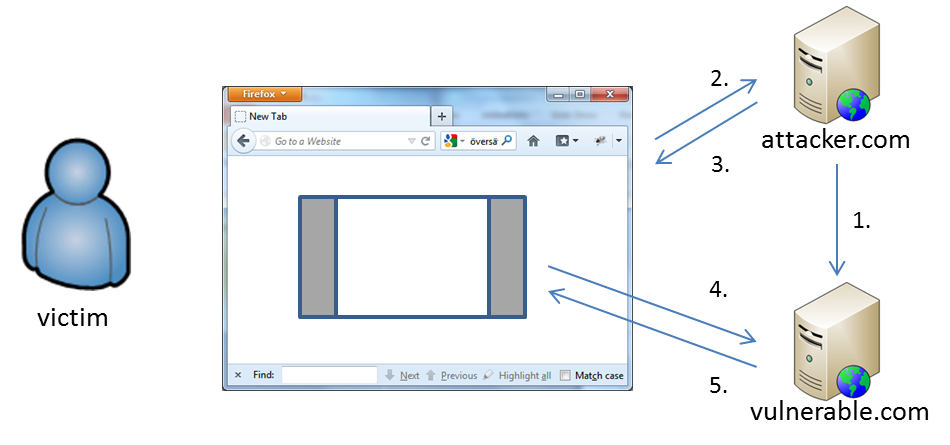
\includegraphics[width=0.49\textwidth]{scenario.png}
  \caption{Overview of the scenario}
  \label{fig:scenario}
\end{figure}

\subsubsection{Syntax injection}
\label{sec:injection}
In a cross-site scripting attack user input is used to compose an HTML document. 
Fragments of HTML syntax in the input alters the semantic of the document to 
execute attacker supplied 
script code. Similarly, in a syntax injection attack the vulnerable target will 
compose an HTML document from attacker controlled input containing syntax of a foreign 
format. The resulting document is a polyglot which is benign when viewed as the 
HTML, but malicious when viewed as the injected format. While the 
web site serves the content as HTML, it is in the hands 
of the attacker to decide how it is interpreted when embedded in the attackers web page. Examples of 
such services include social networks, search engines, i.e., nearly any dynamic web site driven by user interaction.
%
The targeted service is assumed to employ server-side cross-site scripting 
sanitization. For the attack to be successful, the input must 
bypass this sanitization. The sanitization filter will remove or encode 
problematic characters in the input related to HTML-syntax. The injected format will 
pose as a new context, unknown to the filter. Chances are that the 
injected format will pass the filter unnoticed. 

%The polyglot content can
%be interpreted as either the benign original format or the
%malicious attacker-supplied format. 
%

%As an example the
%same-origin policy allows a \emph{script} tag in one document to include JavaScript of
%another origin and execute it in the origin of the document. If an attacker is
%able to inject an HTML document with JavaScript syntax in such a way that it
%became valid JavaScript, the attacker can include the document across origins
%via a \emph{script} tag and extract its content, thereby circumventing the same-origin
%policy.

%The document in Listing \ref{lst:html-js}, is both
%malformed but valid HTML and valid JavaScript in browsers that support
%EcmaScript for XML (E4X). \todo{ref} The
%document can be included as a script in another document and the secret can be
%extracted from variable x. 
%This implies that if an attacker is able to inject
%HTML syntax into a document, closing all previously open tags and
%opening all subsequently closed tags,
%then information can be extracted across origins.
%The injected syntax in the listing is illustrated by highlighting.

%This attack has been suggested as a potential way to bypass Content Security
%Policy~\cite{Heyes:CSP}. As E4X is only supported in the SpiderMonkey JavaScript
%engine, used in Firefox, this limits the exploitability of this example. However,
%this is an unlikely scenario to use JavaScript as the injected format
%because HTML characters are typically escaped by content
%filters. 


Previous work documents an instance of a polyglot attack based on syntax injection, though not phrased in those terms.
Huang et al.~\cite{Huang+:CCS10} describe a cross-origin \emph{cascading style-sheet} (CSS) attack. This 
attack injects fragments of CSS syntax in a HTML 
document, thereby making it a HTML/CSS polyglot. The error-tolerant parsing of 
style sheets allow the polyglot to parsed as valid CSS. The capabilities of CSS 
provide trivial cross-origin leakage. The paper proposes a defense technique which has been
adopted by all major browsers, which implies that the attacks outlined in their paper are now ineffective.
Instead,
Section~\ref{sec:vuln} will show practical attacks based on other formats.


\paragraph{Scenario}
The scenario, illustrated in Figure~\ref{fig:injection-scenario}, describes how 
the attack proceeds from the infiltration of the origin to the compromise of the victim.
Again, the victim is an authenticated user of \emph{vulnerable.com} that 
unsuspectingly visits the attackers malicious web site, \emph{attacker.com} (1). 
The \emph{attacker.com} web site uses a plug-in to embed a web page with 
vulnerable input parameters from \emph{vulnerable.com} (2). 
In the parameters of the request the attacker injects the syntax of the malicious format (3).
The response from \emph{vulnerable.com} is a polyglot served as the benign content type (4), but
the attacker's page coerces the content to be interpreted as the malicious content type by the plug-in.
The malicious payload is executed in the origin of \emph{vulnerable.com} and can 
leverage the credentials of the victim to further exploit the vulnerability.

\begin{figure}[t]
  \center
  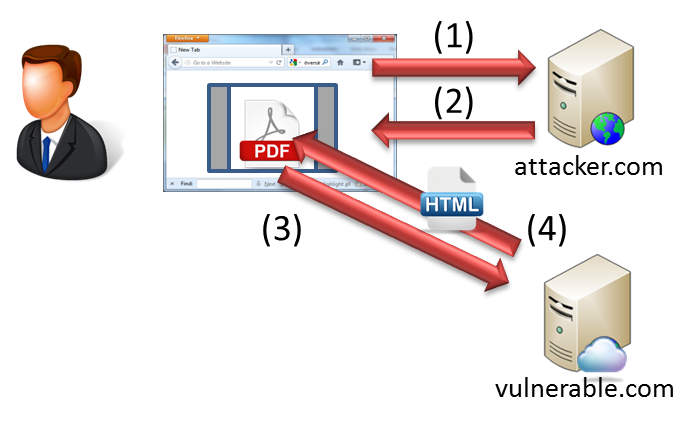
\includegraphics[width=0.49\textwidth]{injection-scenario.png}
  \caption{Syntax injection scenario}
  \label{fig:injection-scenario}
\end{figure}


%\definecolor{lightgray}{gray}{.8}
%\begin{lstlisting}[label=lst:html-js, caption=HTML / E4X Polyglot, escapechar=*]
%<html><body>
%Hello *\colorbox{lightgray}{$<$/body$><$/html$>$;x=$<$html$><$body$>$}*!
%Your secret is 'safe with me'.
%</body></html>
%\end{lstlisting}


\subsubsection{Content smuggling}
\label{sec:smuggling}
The vulnerable target of a content smuggling attack, lets 
users upload files that are subsequently served under the origin of 
the service. Examples of such potentially vulnerable services are cloud storage services, image databases, 
social networks, conference management systems or job broker services. Such a service 
accepts a limited set of benign file-formats, and the files are run through a filter to verify that they 
belong to this set, e.g. images or documents, before being served to the end
user. The
filter will verify the file under the assumption that it conforms strictly to one format. 
By submitting a polyglot to such a service, an attacker can evade the filter as the polyglot does conform to the benign format.
If the polyglot is publicly accessible, it can be embedded in the attackers 
page. Since the attacker is in control over which format the polyglot is 
interpreted as, it is embedded as the malicious format and thereby the 
service is vulnerable to a content smuggling attack.

%a polyglot assuming that it is of the benign format, but once
%the content is served an attacker can coerce the content to be interpreted as
%the malicious format.


The GIFAR attack is a polyglot attack based on content smuggling. In this attack 
a benign GIF-image and a malicious JAR-file is combined to create a GIF/JAR 
polyglot. By submitting the combined GIFAR to a service, the attacker can 
execute a Java applet under the origin of the targeted service. The Java runtime 
has been updated to prevent this kind of abuse.
Instead,
Section
\ref{sec:vuln} will show practical attacks based on other formats.

\paragraph{Scenario}
The content smuggling scenario proceeds as illustrated in Figure~\ref{fig:smuggling-scenario}.
Similarly to the previous scenarios, the victim is an authenticated user of a targeted vulnerable web site, \emph{vulnerable.com}. 
To give more context to the scenario, \emph{vulnerable.com} can be a cloud storage service. 
The target is infiltrated by the attacker (1), who uploads a polyglot to the web site. 
The polyglot is verified to be benign under the assumption that it belongs an allowed file type.
%The \emph{vulnerable.com} site serves the polyglot content as the benign content type, harmless to the victim. 
While still authenticated to \emph{vulnerable.com}, 
the victim visits the attackers web site, \emph{attacker.com} (2).
The \emph{attacker.com} site embeds the polyglot from \emph{vulnerable.com} (3), which is served as the benign type, but 
coerced to be interpreted as the malicious content type by the plug-in (4). 
The malicious format of the embedded 
polyglot is activated and a possible payload is to extract all the files stored in the victims account.

%Other potential targets for this scenario are job broker services and conference 
%management systems, which by design allow submission of PDFs to be viewed by
%users.

\begin{figure}[t]
  \center
  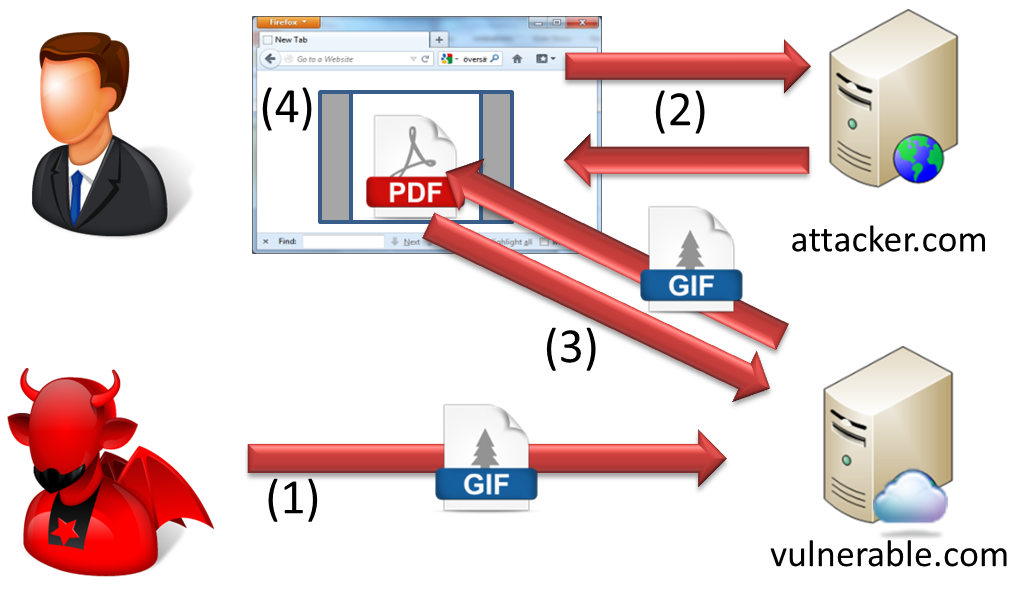
\includegraphics[width=0.49\textwidth]{smuggling-scenario.png}
  \caption{Content smuggling scenario}
  \label{fig:smuggling-scenario}
\end{figure}



\subsection{Payloads}
\label{sec:payloads}
The consequences of exploiting an infiltrated origin depend on the capabilities 
of the format used. These consequences span from abusing the credentials of 
the victim to forge requests to the vulnerable web site, to extracting sensitive 
information about the victim that is stored on the vulnerable web site.

\paragraph{Cross-site request forgery}

If the format has the capability of issuing requests, in particular POST requests
within the boundaries of the SOP, that includes the victims 
credentials,then the attacker can mount a  
\emph{cross-site request forgery} (CSRF) attack. Web sites protect against these attacks by 
generating a token with each response that has to be included in the subsequent 
request. However, if the format also have the capability of reading the response of 
the issued request, it can extract the token and thereby circumvent the CSRF 
protection.

\paragraph{Cross-origin information leakage}

Additionally, if the format allows communication with the origin of the attacker, then 
the attacker can extract sensitive user information and leak it across origins. If the 
format is not restricted by the SOP, it can communicate directly with the 
attackers server. Otherwise, if the format can interact with the document that 
embeds the polyglot, the communication could be tunneled through this channel.






%\subsection{Syntax injection}






%For this attack to be successful certain requirements needs to be fulfilled.
%\begin{itemize} 
%	\item The original content must embed external information under the 
%	control of the attacker. 
%	\item The user-supplied content must circumvent any validation or 
%	filtering. 
%	\item There must exist a way of coercing the resulting polyglot to be 
%	interpreted as the malicious format. 
%	\item The malicious format must have capabilities that are restricted or 
%	missing in the benign format.
%\end{itemize}

% Scenarios

%Much like a cross-site scripting attack, we consider a scenario where a
%web site serves documents which are based upon user-supplied information.

%The same-origin policy is intended to prevent a document from one origin from
%accessing the content of a document of another origin. 


%Consider the php-program in listing \ref{lst:php-sample}. Apart from being
%vulnerable to traditional cross-site scripting, it is vulnerable

%By requesting the site with parameter $guess=</body></html>;x=<html><body>$,
%the resulting document, 



%\subsection{Content smuggling}
% Description of attack technique 

% Building blocks

%The difference in this scenario from the previous one is in the nature of the
%vulnerability. Where in the previous scenario an existing document was injected
%to become a polyglot, this scenario targets services which allow an attacker to
%introduce new documents. As in the previous scenario, the target is a user of
%the vulnerable web site.


%For this attack to be successful, certain requirements needs to be fulfilled.
%\begin{itemize} 
%	\item The service must accept and serve user-supplied files.
%	\item The service must verify the user-supplied polyglot under the 
%	assumption that it is in the benign format. 
%	\item The content is served under the same origin as sensitive user 
%	information.
%	\item There must exist a way of coercing the polyglot to be interpreted 
%	as the malicious format. 
%\end{itemize}

% Scenarios

%3 pages 
\section{Vulnerabilities and attacks}
\label{sec:vuln}

In this section we give concrete examples of the attacks described in 
Section~\ref{sec:cross}, using the PDF format as the running example. We begin
by detailing how the design decision made in the PDF-standard make it highly suitable
for creating malicious polyglots. Throughout this section Adobe Reader is the 
assumed target. A comparison between readers can be found in Section~\ref{sec:eval}.

The reader is invited to visit the test page~\cite{Test:Page:12} for
practical demonstration of the attacks from this section. These
attacks show that the vulnerabilities we focus on are exploitable in practice. 

%\subsection{Concept}

\vfill\eject

\begin{lstlisting}[label=lst:sample-pdf, caption=Sample PDF file]
%PDF-1.4
1 0 obj
<< /Type /Catalog
   /Outlines 2 0 R
   /Pages 3 0 R
>>
endobj
2 0 obj
<< /Type Outlines
   /Count 0
>>
endobj
3 0 obj
<< /Type /Pages
   /Kids [4 0 R]
   /Count 1
>>
endobj
4 0 obj
<< /Type /Page
   /Parent 3 0 R
   /MediaBox [0 0 612 792]
   /Contents 5 0 R
   /Resources << /ProcSet 6 0 R >>
>>
endobj
5 0 obj << /Length 35 >>
stream
   ...Page-marking operators...
endstream
endobj
6 0 obj
   [/PDF]
endobj
xref
0 7
0000000000 65535 f
0000000009 00000 n
0000000074 00000 n
0000000120 00000 n
0000000179 00000 n
0000000300 00000 n
0000000384 00000 n
trailer
<< /Size 7
   /Root 1 0 R
>>
startxref
408
%%EOF
\end{lstlisting}




\subsection{Portable Document Format}
\label{sec:format}
% Why PDF format?

The \emph{Portable Document Format} (PDF) is a widely used document format 
capable of displaying text, rendering graphics, scripting, animation and other 
dynamic content. It is a container format in the sense that it allows 
embedding of files and resources.

According to the PDF specification~\cite{PDF:ISO08} a PDF file is composed of
a header, several objects, a cross-reference section and a trailer. Listing~\ref{lst:sample-pdf} 
shows a sample of how a PDF file is structured and its elements. Supposedly, it is also a minimal PDF file according to the specification.

% header
\subsubsection{Header}
The header consists of the string "\%PDF-" followed by a version number. 
The version is denoted by a 
major and a minor version number of the form "\emph{M.m}". Because the version can 
be specified elsewhere, the version number is not required to be part of the 
header.


% objects
\subsubsection{Objects}
Objects can be direct or indirect, the difference being that an indirect object 
has labels which are used for referring to the object from another object. Object 
labels are numbered and begin with the string "\emph{N n} obj", where "N" is the object number and "n" is the 
revision number. Similarly object references are of the form "\emph{N n} R".
The label is optionally ended with the keyword "endobj".

There are eight basic types of basic objects; booleans, integers, strings, names, 
arrays, dictionaries, streams and the null object. For the intents and purposes 
of this article, we will focus on the string, dictionary, name and stream objects.

% string objects
\paragraph{String objects}
There are two types of strings; literal and hexadecimal. Literal strings are 
enclosed by the "(" and ")" characters. Any character can occur in a literal 
string, even parentheses if they are balanced, e.g. a matching closing 
parenthesis for every opened parenthesis. In hexadecimal strings 
each character is represented by its corresponding hexadecimal value, enclosed 
by the "$<$" and "$>$" characters.

% dictionary objects
\paragraph{Dictionary objects}
Dictionary objects are a name-value map delimited by the "$<<$" and "$>>$" 
tokens. The names are name objects and the values are objects of any type.
% name objects
Name objects begin with the "/" character, followed by a string of non-whitespace 
characters. Each dictionary has a type, either specified by the "/Type" name or inferred 
from the context in which it occurs. The type declares which kind of element the 
dictionary is describing, e.g. a page or an annotation. Dictionaries form the structure of the document by connecting
objects through references, e.g. relating a page to its contents. %At least one 
%dictionary is required to build a PDF document. 
% actions?
A special type of dictionary describes \emph{actions}. Actions are triggered when a
certain event occur, such as a file is opened or a page is displayed, and the action 
dictionary specify how it is handled. Actions can be used to, among other 
things, go to a specific page, play a sound, execute JavaScript or launch a command.

% stream objects
\paragraph{Stream objects}
A stream is an unlimited sequence of bytes. A stream object is indirect and consists of a 
dictionary, describing the stream, and the associated stream delimited by the 
"stream" and "endstream" keywords. 
%
According to the specification, the stream dictionary shall contain a \emph{Length} 
name to specify the length of the stream. In practice this can be omitted as 
long as the delimiting keywords are in place.
%
PDF supports encoding of streams, in which
case the dictionary describe which filters are required to decode the stream. 

% cross-reference
\subsubsection{Cross-reference}
The cross-reference section is a record of the location of indirect objects 
within a file. The location is specified as the byte offset from the beginning 
of the file. The cross-reference section is opened with the "xref" keyword,
followed by one record for each indirect object. The cross-reference section 
will be reconstructed if missing and can therefore be omitted.

% trailer
\subsubsection{Trailer}
The trailer is composed of a trailer dictionary, a pointer to the cross-reference 
section and an end-of-file marker. The trailer dictionary is introduced by the 
"trailer" keyword. 
%
\emph{Root} is in practice the only mandatory name in the trailer dictionary, referencing the root of the 
%
document structure. The "startxref" keyword is followed by the number of bytes from 
the beginning of the file to the first cross-reference section. As with the 
cross-reference section, it can be omitted. The string "\%\%EOF" marks the 
end-of-file, but can be omitted.


\subsection{PDF-based polyglots}
\label{sec:pdf-based-polyglots}
Several design choices in the PDF specification make the format particularly 
suitable for making polyglots. One such design choice is the error tolerant 
parser. This is in part motivated by another design choice namely PDF being a container format. 
%of which the 
This implies
%implication is 
that a PDF file can, by design, contain foreign syntax that 
could interfere with the syntax of the file. Another motivation is that PDF 
files are designed to be both forward- and backward-compatible. Readers 
implementing an older version of the specification do not recognize new 
features and behave as if they were not present in the file. 
%
The implementation notes of the specification describes some exceptions to the
requirements of the specification, such as the header can occur 
anywhere within the first 1024 bytes of the file. This flexibility gives plenty of room for 
combining with syntax of another format.
%
The specification declares many components to be required in a
PDF file, but as can be seen in Section~\ref{sec:format}, in practice several 
components can be omitted~\cite{Wolf:CCC10}. The code in Listing~\ref{lst:minimal-pdf} shows the 
minimal syntax required for a malformed, but valid PDF file.
%incrementally 
%updated by appending updated versions of existing objects to 
%the end of the file. In fact, 
%and formats. This and the fact that it is designed to be robust against errors,
%provides us with a format that is powerful, flexible and ideal for creating
%malicious polyglots.


\begin{lstlisting}[label=lst:minimal-pdf, caption=Minimal PDF file]
%PDF-
trailer<</Root<</Pages<<>>>>>>
\end{lstlisting}

% - Execute JavaScript
% - Embed Flash files
% - Launch commands
% - Network requests

Furthermore the PDF format is of particular interest to us because of its 
many capabilities. Some examples include executing JavaScript, launching commands, 
and issuing HTTP requests. The HTTP requests are restricted to the origin of the 
PDF file, and will include any cookies associated with that origin. 
Adobe Reader also includes a Flash 
runtime to play embedded Flash files on systems that do
not have the Flash runtime installed. %Considering that it might be a conscious decision
%of the user to refuse a flash player, 

%\subsection{Embedded PDF documents}

When a PDF document is embedded in a web page, the corresponding plug-in 
is executed to render the content. Recall from Section~\ref{sec:cross-origin} 
that the plug-in is selected based 
on the MIME-type, either supplied by the server or in the type attribute
%
with preference for the later.
%
Also recall
that the browser rely on the plug-in to handle the situation when the MIME-type 
supplied by the server is inconsistent with the MIME-type of the plug-in.
In the case of the Adobe Reader plug-in, it disregards the MIME-type
supplied by the server and will attempt to interpret any content as PDF. 
Listing~\ref{lst:embed-pdf} shows how 
arbitrary content can be rendered as PDF format.


\begin{lstlisting}[label=lst:embed-pdf, caption=HTML for embedding PDF content]
<embed type="application/pdf" 
src="vulnerable.com/?input=%PDF...">
\end{lstlisting}


In recent versions of Adobe Reader certain measures have been taken to prevent 
creating PDF-based polyglots. In accordance with our recommendations, Adobe Reader 
has made the parsing more strict by attempting to match the first bytes of the 
file against a set of known signatures. If 
a match is found, the parser will abort loading of the document. 
However, this does not fully defend against PDF-based polyglot attacks.
The problem of 
this approach is that there are a number of file formats that lack a reliable 
signature, e.g., HTML. Also, for this approach to be reliable, the signature 
must match the signature enforced by other interpreters of the format. A notable 
counterexample is the signature used for the JPG format. While the signature is 
correct according to the specification of the format, several JPG interpreters
will allow slightly malformed signatures. Such a malformed signature will bypass 
the check in Adobe Reader and still be rendered correctly in a viewer. This opens up for PDF-based
polyglot attacks.

\subsection{PDF attacks}

As explained in Section~\ref{sec:vectors} there are two vectors for polyglot 
attacks; \emph{syntax injection} and \emph{content smuggling}. PDF is a suitable 
format for both vectors as it is both a text based format with error tolerant parsing, 
and has widespread acceptance as a document format, often preferred over 
other document formats.

\subsubsection{Syntax injection}
\label{sec:pdf-injection}
As the scenario details in Section~\ref{sec:injection}, the attacker in a syntax 
injection attack manipulates a vulnerable service to include PDF syntax in existing content, e.g. HTML-documents.
The PDF syntax is typically injected through user input used by the vulnerable service in the composition of documents.
%
An example of a suitable fragment to inject is shown in Listing~\ref{lst:xml-pdf}.
%
The resulting content is subsequently 
embedded in the attackers page as PDF, as exemplified in Listing~\ref{lst:embed-pdf}.
As mentioned in Section~\ref{sec:pdf-based-polyglots}, the embedded PDF can issue 
requests to the origin it came from, carrying the cookies associated with that origin.
These requests allow for the extraction of sensitive user data that can either be 
communicated back to the attacker, or be leveraged in further attacks.

Thus far, exploitation of vulnerable services have been discussed, excluding the specific 
conditions under which a service is vulnerable. In order to exploit the 
vulnerability, the injected syntax must pass through any existing filters 
unchanged or at least with its semantics preserved. If user input in an 
HTML-document is not sanitized, any syntax would be unchanged and 
the service is vulnerable to less sophisticated attacks, e.g. cross-site scripting, 
therefore sanitized user input is of greater concern.
%
Based on the PDF samples in Listings~\ref{lst:minimal-pdf} and~\ref{lst:xml-pdf}, we can derive 
the set of tokens required to build a PDF. Assuming that alpha-numeric characters 
pass through a sanitization filter unmodified, the set of tokens is $\{\%, <<, >>, /\}$.
As can be noted, there is a small but significant overlap with the tokens of HTML, 
which implies that many web sites protected against cross-site scripting attacks 
are also protected against PDF-based polyglot attacks. One of the problems of 
filtering input for inclusion in a web page are the many contexts in which the 
input can be included. A problem made even more complex by the diversity of 
languages the page contains. Language incompatibilities force context dependent 
filtering, where the same input is treated differently based on the context in 
which it is included. In certain contexts angle brackets are often left untouched by filters.

\paragraph{HTML comments}
No HTML enclosed in comments, "$<$--" and "--$>$", will be rendered, and therefore 
filters consider this context safe. To prevent input from escaping the comment by 
injecting an end comment token, certain filters remove any occurrences of "--$>$", 
but leave the rest of the input untouched. HTML comments are meaningless to PDF, 
and the result is a valid HTML/PDF polyglot.

\paragraph{JavaScript strings}
In an in-line JavaScript context, user input is often included in the shape of a 
JavaScript string, delimited by single or double quotes. In this context only a 
few characters require encoding, as they can break the string context. Naturally, 
any single or double quotes need escaping, as well as any carriage return or 
line feed characters. In the spirit of making minimal changes to the input, 
certain web sites only escape these characters. This is sufficient to prevent cross-site 
scripting attacks, but fail to protect against PDF-based polyglot attacks.

Note that not only in-line JavaScript falls short in this regard. JavaScript object notation 
(JSON) is used in modern web sites as a data transport. This is particularly 
common in web sites that provide an API to interact with the offered services.
JSON encoded information suffer the same problem as in-line JavaScript, thereby
extending the attack surface further.

\subsubsection{Content smuggling}

Due to the nature of the PDF, it can without much effort be combined with just 
about any other format. This provides ample opportunity to create malicious 
polyglots where PDF is either the benign or the malicious format. Consequently, 
this significantly expands the attack surface, making it important to take 
measures to protect against these attacks.


\paragraph{PDF as the benign format}
%\todo{Services that accept PDFs, PDFs can be used to hide another malicious format}
Services like job brokers commonly let the user upload a CV in the form of a PDF-file.
Before such PDF-files are published to recruiters, they are verified to not 
contain any malicious payload. Such a verification only extends to the PDF format itself.
An attacker can produce a PDF that is valid and 
benign, but also a polyglot hiding another malicious format, such as Flash. As 
described in the content smuggling scenario in Section~\ref{sec:smuggling}, the 
uploaded PDF file is then embedded on the attacker's web site, but now as the 
malicious format. Using social engineering, the attacker can persuade 
the victim to visit the web site.

Creating a PDF/Flash polyglot is no major challenge.
A proof-of-concept can easily be created by storing the PDF source code as a static string 
variable in the malicious Flash source code. When compiling Flash, the output is 
compressed by default to save space, thereby obfuscating the PDF source code. However, tools exist 
that decompress the Flash files, which restores the plain PDF code.

\paragraph{PDF as the malicious format}
In the content smuggling scenario in Section~\ref{sec:smuggling}, the 
attacker uploads the PDF polyglot to a vulnerable content hosting service. 
A server-side verification process will base its verification on the benign formats 
it expects to receive. The polyglot is designed to verify correctly as the benign format,
and the verification is likely to miss the malicious PDF components, as it is unaware of the alternate interpretation of the content. 

Given the extensive capabilities of the PDF format, exploiting a content smuggling 
vulnerability with a PDF-based polyglot attack, can be done without much effort.
To prevent the attack, the 
verification process have to actively search for and remove PDF specific syntax.
The impact of exploitation depends on the payload used in the attack.

\subsection{PDF payloads}
%\todo{rewrite section, focus on embedded flash, xxe and code samples}
%
As discussed in Section~\ref{sec:payloads}, there are two approaches to exploiting 
these vulnerabilities; cross-site request forgery, and cross-origin information leakage.
Both of these require extracting information from the vulnerable service, which is something that can be achieved using the capabilities of the PDF format.

In order to extract information and leak across origins, a communication channel
is established. PDF documents provide multiple ways of generating HTTP requests; 
many of which allow cross-origin communication, but are, out of security concerns, only one-way in the sense that 
the PDF document will never see the result. Therefore, the focus is directed towards 
two methods that allow bidirectional communication; XML external entities, and embedded Flash. 
 Since the document will retain the 
origin from which it was served, all 
requests issued from the document will include any cookies associated with the target origin.

%When embedded in a web page, many of the PDF communication methods utilize
%the underlying browser to make requests by navigating the browser to the target 
%URL. This will unload the current page in which the document is embedded. Arbitrary page 
%navigation is allowed with respect to SOP, since the response is not visible 
%to the document. Such methods can be used in CSRF attacks, but would 
%defeat the purpose of requesting information as the document cannot process the 
%response.

% Cross-origin leaks
%To leak information across origins, a communication channel is 
%required between the attacker and the target. PDF provides the necessary means 
%to mediate this information leakage. The flow of information can be divided into 
%two steps, extracting information from the target and delivering it to the attacker.
%Each requiring its own communication methods.


%\subsubsection{The target}
%There are two methods for a PDF file to communicate with the server it originates from, 
%both allowing it to read the response: from JavaScript using XML external entities 
%and from an embedded flash file.

\paragraph{XML External Entities}
The PDF JavaScript API includes a method to parse XML documents, called 
XMLData.parse. The XML document being processed may in turn rely on external entities, 
required for the parsing of the document, which the XML parser will request. The request is 
bound to the origin of the document, and the response is included in the XML document. 
The source code of the XML document reflects this response and can be retrieved at a later point,
resulting in a bidirectional communication channel.
%
As the response 
is included in the XML, the result has to be well-formed XML. This puts a 
restriction on the content that can be requested using this method. Considering 
that HTML pages are rarely well-formed this method may be too restricted in practice.

Listing~\ref{lst:xml-pdf} contains an example PDF document that uses XML external 
entities. The one-way method \emph{getURL} is used to communicate the 
information back to the attacker. Given the compact size of the example, it is useful for the syntax 
injection scenario in Section~\ref{sec:injection}, which require injection of 
small syntax fragments.

As of version 10.1.5, in accordance with our recommendations,  XML external entities 
has been removed. Thereby the risks of leakage of sensitive information is significantly reduced.


\paragraph{Embedded Flash}
By embedding a Flash file in the PDF document the capabilities of the format can be 
extended even further. The Flash runtime supports bidirectional communication in 
accordance with SOP.
%
The embedded Flash inherits the origin of the PDF document, thus it can 
request and read any document from the originating server. Unlike the XML
method, there are no restrictions on what content can be requested, thus making 
it the most versatile of the available communication methods. The only drawback 
using this approach is the significant increase in terms of file size. Even the compact 
Flash code in Listing~\ref{lst:flash-pdf} will result in a 6 kB Flash file. 
This suggests that this method might be better suited for the content smuggling 
scenario in Section~\ref{sec:smuggling}, rather than the syntax injection scenario.

Cross-origin communication in Flash adheres to the same-origin policy. However, this is not a restriction, since
 Flash also supports cross-origin communication via  
cross-origin resource sharing. Using CORS, a web server can relax the SOP to allow access to specified content.
%As mentioned, the embedded Flash file inherits the origin of the document.
An attacker can set an allow-all cross-origin policy, such as in Listing~\ref{lst:crossdomain}, 
that open up for two way communication.


\begin{lstlisting}[label=lst:xml-pdf, caption=PDF using XML for communication]
%PDF-
1 0 obj<<>>stream
xml = '<!DOCTYPE foo[<!ENTITY x ' +
 'SYSTEM "'+URL+'">]><foo>&x;</foo>';
var doc = XMLData.parse(xml);
getURL('attacker.com/?secret='+
  doc.saveXML())
endstream
trailer<</Root
   <</Pages<<>>
      /OpenAction
      <</S/JavaScript/JS 1 0 R>>
   >>
>>
\end{lstlisting}

\begin{lstlisting}[label=lst:flash-pdf, caption=Flash code for communication]
package {
  import flash.net.*;
  import flash.display.Sprite;
  public class Secret extends Sprite {
    var u:String;
    var r:URLRequest;
    var l:URLLoader;
    public function Secret() {
      u = 'vulnerable.com/secret';
      r = new URLRequest(u);
      l = new URLLoader(r);

      l.addEventListener('complete', 
        function():void {
          u = 'attacker.com/?' + r.data;
          r = new URLRequest(u);
          l = new URLLoader(r);
        });
}}}
\end{lstlisting}

\begin{lstlisting}[label=lst:crossdomain, caption=Allow-all crossdomain.xml]
<cross-domain-policy>
  <allow-access-from domain="*" />
</cross-domain-policy>
\end{lstlisting}

%\subsubsection{The attacker}
%There are a number of ways to communicate with the attacker, either directly 
%via the embedding page or through the attackers server. As mentioned previously, 
%many methods trigger page navigation in the browser. This will result in a 
%noticeable change in the victims browser. While it fulfills the purpose of 
%leaking information, an attacker can use more covert methods of communication
%to refrain from alerting the victim. 

%\paragraph{Fragment identifier}
%The methods that navigate the browser can still be used for a somewhat covert 
%communication with the attacker. Navigating to the same page with a different 
%fragment identifier will not reload the page. Embedding the information in the fragment 
%identifier of the URL of the embedding web site, creates a one-way communication 
%channel from the document to the page. Since the fragment identifier is visible 
%in the address field of the browser, an alert user would notice it changing.

%\paragraph{PostMessage}
%The PDF plugin includes an API for communicating directly with the page in 
%which it is embedded. The document can send messages to the page using 
%the hostContainer.postMessage method. The page registers a handler to receive 
%the event and is also able to post messages back to the document.
%This two way communication is not visible to the victim.

%\paragraph{Embedded Flash}








%3 pages 
\section{Evaluation}
\label{sec:eval}

This section details the evaluation performed to investigate the prevalence of 
the vulnerabilities from Section~\ref{sec:vuln}. The evaluation covers various 
instances of affected components, such as browsers and PDF interpreters, 
content sanitization filter, and a study of the Alexa top 100 web sites.

\subsection{Instances}

To better understand how this problem presents itself, a comparison of browser and reader instances 
is presented. We compare all major browsers and two of the most common readers.

\subsubsection{Readers}
\label{sec:readers}
Section~\ref{sec:vuln} focuses on the Adobe PDF Reader as the attack surface, 
due to its standing as the most commonly used reader. To give a comparison, the 
Google Chrome built-in PDF reader was selected as it is the default reader to 
users of the browser.

As mentioned in Section~\ref{sec:cross}, the browser rely on the reader plug-in to 
implement correct security measures, in order to prevent cross-domain leakage. 
Unlike Adobe Reader, the Chrome browser built-in PDF reader refuses to render 
content that was served with an inappropriate MIME-type if the content is 
delivered across origins. This effectively prevents the attacks in Section~\ref{sec:vuln}.
If the Chrome browser is configured to use the Adobe Reader plug-in, it will 
behave the same as in other browsers and the content will be interpreted as PDF.

\subsubsection{Browsers}

The behavior of cross-domain embedding of PDF resources is studied in the major 
browsers, i.e., Firefox, Safari, Opera, Google Chrome and Internet Explorer. 
The study shows that all major browsers are susceptible to the attacks outlined 
in Section~\ref{sec:vuln}, with some minor differences detailed below and summarized in Table~\ref{tab:comparison}.
In Table~\ref{tab:comparison}, "Yes" for the columns "object" and "embed" indicates that the 
corresponding tag can be used to embed a PDF document, and for the column 
"Adobe is default" it indicates that Adobe Reader is commonly the default PDF reader.

\paragraph{Firefox, Safari and Opera}
The browsers, Firefox, Safari and Opera, are all susceptible to the attacks outlined as 
per Section~\ref{sec:vuln}, without any restrictions or modifications.

\paragraph{Google Chrome}
Google's browser, Chrome, has built-in support for displaying PDF documents. 
The built-in PDF reader is used by default by the browser, unless it has been 
explicitly disabled by the user. Certain complex PDF documents can not be 
handled by the built-in reader. The built-in reader will then prompt the user 
to open the document in Adobe Reader. As previously noted in Section~\ref{sec:readers}, the built-in reader 
is not vulnerable to attacks. Hence, Chrome is only susceptible when the Adobe 
Reader plug-in is used to render the document.

\paragraph{Internet Explorer}
Microsoft's browser, Internet Explorer, is susceptible to the attacks. However, 
it seems to only support embedding of PDF documents using the \emph{embed} tag. 
This is not a major obstacle in exploiting the vulnerability, as the \emph{embed} and 
\emph{object} tags are interchangeable in this respect.

\begin{table}[t]
\begin{tabular}{l|c|c|c}
& object & embed & Adobe is default \\ \hline
Firefox & Yes & Yes & Yes \\ \hline
Chrome & Yes & Yes & No \\ \hline
Safari & Yes & Yes & Yes \\ \hline
Opera & Yes & Yes & Yes \\ \hline
Internet Explorer & No & Yes & Yes %\\ \hline
\end{tabular}
\caption{Comparison of browsers}
\label{tab:comparison}
\end{table}
%\subsection{Bypassing content filters}


%\subsubsection{Server-side upload filters}

%As discussed in Section~\ref{sec:cross} server-side content filters that 
%validate files based on content type are not equipped to handle polyglot 
%content. For polyglot content, specialized filters are required that analyze 
%the content based on all considerable interpretations of the content. No such 
%filters were encountered in this study.

%\subsubsection{Cross-site scripting filters}
%\todo{install NoScript?}
%This effectively bypasses any cross-site scripting filters such as NoScript or
%filters built into browsers. Since the Reader plug-in handles the response, the
%browser never gets to see the content


%\subsubsection{Context sensitive filters}

%Context sensitive cross-site scripting filters, that remove or encode characters
%Clever filters that adapt their filtering to the context in which the user
%content is included. Basically filters that allow input that do not form harmfulHTML.

% Don't want to claim something I have no basis for..

\subsection{Alexa top 100}
We have conducted two
studies to evaluate the prevalence of the problem on popular sites, 
covering the Alexa top 100 web sites. Because of their dominance 
on the web, these web sites are also the most exposed to security threats.
The first study covers PDF-based polyglot attacks using syntax injection as the 
infiltration method; the second covers content smuggling.
%It does not involve polyglot attacks based on content smuggling, as 
%potential targets generally require authentication before submitting content.
We refrain from mentioning names of individual web sites to prevent exploitation 
before the issues have been properly dealt with.
We are in contact with the maintainers of the web sites to help
mitigate the vulnerabilities. 


\paragraph{Syntax injection}
The study is based on supplying the web sites with the benign minimal PDF in 
Listing~\ref{lst:minimal-pdf}, and examining the corresponding responses to this input.
The sample contains the essential keywords and tokens required to perform a syntax 
injection based polyglot attack. If these tokens pass through unaltered, the web site is 
considered vulnerable. The process has been conducted manually and only input 
parameters on publicly accessible pages, those that do not require authentication, 
were tested. Considering that most inputs are available only to authenticated 
users, the results suggests that more web sites are likely vulnerable in input that do
require authentication.

The conclusion is 
that nine web sites out of the hundred apply insufficient content filtering with 
respect to the PDF format. Out of the nine found to be vulnerable; five were 
susceptible to PDF based polyglot attacks, and four applied 
insufficient content filtering, but the input was reflected in a way that 
prevented exploitation, e.g. the header appeared after 1024 bytes.
%
%, which have the potential of compromising the 
%confidentiality and integrity of the web site's users.
%

Three of the five vulnerable web sites could also be determined to be vulnerable to 
traditional XSS attacks in the same input parameters. 
The remaining two web sites found susceptible only to polyglot attacks and not XSS attacks
are of particular interest since they employ proper measures to protect 
against XSS attacks, and yet fall short in defeating this new breed of attacks.

\begin{enumerate}
\item The first web site reflected user input in an inline  
JavaScript context, inside a string. To prevent cross-site scripting in this 
context, the following measures were taken: the JavaScript string delimiters 
and the backslash character were properly escaped, and the 
string "$<$/script$>$" was removed. These measures are sufficient to protect against XSS attacks, 
but do not prevent an attacker 
from injecting valid PDF syntax.
\item The second web site reflected the user input in an HTML-comment context. 
The only measure taken to prevent XSS attacks in this context was removing any 
occurrence of the character sequence "--$>$". Again, while successfully preventing 
XSS attacks, this measure is ineffective in preventing an attacker from injecting PDF syntax.
\end{enumerate}

\paragraph{Content smuggling}
Further, a smaller study was conducted, not covering the full Alexa top 100, but 
targeting popular cloud storage services. 
This study is based on polyglot content being uploaded to the service and 
subsequently analyzed to determine which origin it was served 
under. We have found two major 
enterprise cloud storage services to be susceptible to attacks. Both services make an effort to
follow current best practices, see Section~\ref{sec:smuggling-mitigation}, but 
fail to cover certain scenarios for content upload. 

The first service serves almost all uploaded content from a sandboxed origin; the exception being the user's 
avatar image that are served under the sensitive origin. An attacker could 
upload a specially crafted avatar image that, when embedded as PDF on the attackers 
web site, can access and modify the contents of the victim's cloud storage.

The second service lets the user publish a public link to an HTML 
representation of the content. The content is served under the sensitive origin 
and is therefore carefully processed to prevent 
generation of malicious HTML, but fails to take other formats into account.
A specially crafted file will result in the generation of valid PDF syntax that, when embedded as PDF on the attackers 
web site, can access and modify the contents of the victim's cloud storage.

We are currently advising both service providers to help mitigate these vulnerabilities. 

%Baidu.com (allows <>, but escapes /) 
%LinkedIn (allows <>, but escapes /) 
%Soso (allows <>, but escapes /) 
%Youku (vulnerable to traditional XSS) 
%Soku (vulnerable to traditional XSS) 
%alibaba.com (allows <>, but escapes /)
%about.com (vulnerable to traditional XSS,
%http://linux.about.com/sitesearch.htm?q=XSS&SUName=--%3E%3Cimg+src=x+onerror=alert%281%29%3E)
%sogou.com (potential target
%http://www.sogou.com/web?query=%25PDF+%3C%3C+%2F+%3E%3E&_asf=www.sogou.com&_ast=1349689275&w=01019900&p=40040100&sut=11010&sst0=1349689274528)





%1-2 pages 
\section{Mitigation}
\label{sec:mit}
This section gives advice on various mitigation approaches available for each of the
affected components, both server-side and client-side. 
We provide one general mitigation approach that covers a significant segment of 
the potential attack vectors, and provide specific mitigation suggestions for affected 
components.

Although some of the mitigation suggestions below are already in place
(e.g., the Chrome builtin PDF reader), the state of the art
is far from being satisfactory. As our paper demonstrates, the
polyglot attacks are a real threat. It is the paper's main value to
bring attention to polyglot attacks and the importance of
mitigation against them.

\subsection{General approach}
It should be noted that 
preventing polyglots, and thereby polyglot attacks, in the general case is a complex task, as one would 
need to take all potentially malicious formats in to account. Mitigating instances of 
polyglot attacks based on particular formats are significantly more straightforward. 
Our approach is not attempting to prevent polyglots as such, but provide details about 
the context in which the content will be interpreted, such that an informed decision 
can be made on whether rendering the content constitutes a security risk or not.

The relation between web server and the browser is central in a web environment, but 
there is no common agreement on the type of content communicated between server 
and client. As mentioned in Section~\ref{sec:cross-origin}, in each response the web server sends a 
header representing its view on the type of content delivered, however, the browser
is free to ignore the provided type and can even be instructed to do so.
Often the browser knows precisely the context in which the content will be 
rendered and the types suitable for these contexts. 
%
As an example, when content is loaded in an \emph{object} tag with a type attribute, as 
is the case throughout the paper, the browser already
has exact knowledge as to which types the requested content can be interpreted as in this context. A natural
defense technique is to send the expected types along with the request. The web server
then compares the expected types to the assumed type and react accordingly, e.g., 
if the assumed type is HTML and the expected type is PDF, an 
error can be sent back to the client. On the client side, the browser verifies 
the type in the response matches any of the expected types, possibly alerting 
the user if there is a mismatch. This mutual agreement between client and server
can help mitigate both syntax injection and content smuggling.
Furthermore, this approach can be implemented in the
web server itself, as opposed to a web application, since the web server makes the
final decision on the supplied content-type. 

The expected type is useful also to a web application that performs content 
filtering on the fly. At the point when the content is being requested, it only 
requires verification against the expected type.

There are limitations to this technique; If a context has multiple
possible types, e.g., an \emph{img} tag, 
a polyglot between two of the types can evade detection. The specific cases where this situation 
occurs in an exploitable way are rare, and further work can help in determining and mitigating such 
vulnerabilities. 

\subsection{Specific approaches}

Apart from the general approach described above, there are mitigation approaches 
that are specific to each of the components involved. These are recommended to 
be used until general approaches for mitigating polyglot attacks are widely adopted.

\subsubsection{Server-side mitigation}

As a content provider on the Internet today there are precautions that one can 
take to mitigate this class of vulnerabilities. Which precautions to take depend 
on the kind of services provided. The mitigation recommendations for syntax 
injection apply to all services that generate content based on user input, and the content smuggling
recommendations apply to services that serve user-supplied files.

\paragraph{Syntax injection}

%In the case of PDF; always encode tokens related to the PDF 
%syntax. Generally, hard to ensure that tokens for all potential 
%file formats are properly encoded without breaking anything.

Preventing syntax injection on the server-side poses severe challenges.
Even server-side filtering of HTML syntax to prevent cross-side scripting
attacks has proved difficult due to the many contexts in which JavaScript can be 
introduced. Filtering all potentially harmful tokens from all formats in which a 
document may be interpreted is hardly possible.

To prevent attacks based on a specific format, e.g., a PDF-based syntax injection attack, the task is simpler. As discussed in Section~\ref{sec:pdf-injection}, the token-set identified in 
Section~\ref{sec:pdf-injection}, are essential 
to create valid PDF syntax. %, namely \emph{'$<$', '$>$', and '/'}.
Filtering 
user input to remove or encode these characters effectively mitigates the 
vulnerability. 
Luckily, because of the significant overlap with the token-set
of HTML, many of the contexts where user input can occur are already being protected.
Special attention is required in contexts are not traditionally filtered for 
HTML tokens, e.g. JSON.

\paragraph{Content smuggling}
\label{sec:smuggling-mitigation}
The current best-practice recommendation
on hosting user-supplied content 
is to serve the content from a sandboxed origin that is 
completely separate, as per SOP, and isolated from the sensitive services. 
These best-practices, provided by Google~\cite{Google:ContentHosting}, successfully prevents content smuggling 
attacks as the restrictions of the SOP prevents the content from accessing any sensitive 
resources in the origin of the web service.

These recommendations come with a caveat to be taken into consideration. Some user supplied 
content is only meant to be accessible to certain authenticated users, e.g. photos that 
are only shared with friends. In that case, the service needs to transfer the 
credentials required to authenticate the user from the sensitive origin to the sandboxed 
origin, without actually revealing the credentials used in the sensitive origin. 
Revealing the credentials, e.g. using the same cookies on both origins, defeats 
the purpose of the sandbox origin entirely. Currently there is no uniform solution 
to this problem. Some common solutions are encountered: using the hashed 
credentials of the sensitive origin; or generating public, but obscured, links 
that are later shared manually.


%\todo{Problem of transferring credentials between domains for services where the content requires authentication}

%Google uses the domain name \emph{googleusercontent.com} to sandbox all the 
%untrusted user files that their various services provide for their customers.


\subsubsection{Browser}

Traditionally, browser vendors have allowed the browser to override the 
MIME-type provided by the server for compatibility reasons. This is a compromise 
to deal with the situation that the server is confused as to what kind of content it is serving. This compromise 
has repeatedly shown to lead to security issues. The affected browser vendors 
can help mitigate this problem by limiting the ways content can be coerced to be 
interpreted as a particular format.

In the case of PDF-based polyglots, and other polyglots that require a plugin, the browser can intervene when there is a 
mismatch between the content-type provided by the server and the type attribute 
of the \emph{object} tag. The vulnerability can be mitigated by acknowledging that there is a potential security issue in 
interpreting the supplied content in the requested format and alerting the user to this
threat.

An intuitive approach would be to for the browsers to employ similar content-sniffing
for content rendered in plug-ins, as is already done with content native to the browser.
However, this intuition fails to take into account that the very reason for using plug-ins 
is that the format is unknown to the browser. 
One may argue that the browser is as confused as the originating server as to the 
actual format of the content, and that the issue would be best resolved by the 
corresponding plug-in.

\subsubsection{Interpreter / Plugin}

As a general rule of thumb, the interpreter must at the very least alert the user if the served 
content-type differs from the expected. A preferred alternative is to 
not attempt to interpret the content at all. This holds true especially when 
the served content-type is well known and radically different from that which 
the interpreter is designed for.

As for the PDF file format, the underlying design decisions have led to the 
current parsing being very relaxed. 
As discussed in Section~\ref{sec:pdf-based-polyglots} the PDF format is a container format; designed to 
embed syntax from other files. 
Even when parsing strictly according to 
the specification, it is a simple task to create a PDF-based polyglot.
Making the parsing more strict and enforcing many of the specified requirements 
will make it harder to create polyglots, reducing the attack surface. 
In accordance with this recommendation, Adobe has taken the first 
steps to prevent PDF-based polyglots. Recent versions of the reader compares the first 
bytes of the document against a set of known file signatures.
While this is a step in the right direction, this kind of black listing has its drawbacks.
The difficulty is that a number of file formats that lack a reliable 
signatures, e.g., HTML.

A different approach is restricting capabilities of the format, sticking to the 
essential features. The more capable the format is, the more likely it is to 
introduce security flaws. In the latest version of their reader Adobe has made 
progress also in this respect 
by restricting the possibilities for bidirectional communication.



%1 page 
\section{Related work}
\label{sec:related}
Recall that the added value of our paper is a generalized account of polyglot attacks and focus on new
instances of polyglots that involve the PDF format. We briefly report
on related instances of polyglot attacks.

Backes et al.~\cite{Backes+:SP07} explore the power of the PostScript
language. PostScript allows executable content and access to sensitive
information from the environment such as the user id. This work
demonstrates how to compromise reviewer anonymity in a peer-reviewing
process by maliciously crafting a PostScript document.

As discussed in Section~\ref{sec:cross}, 
GIFAR~\cite{Brandis:GIFAR} is based on polyglots that combine the GIF and JAR (Java
archive) formats. The former is used as benign and the latter as
malicious to bypass SOP. The Java virtual machine vendors have since
then mitigated these attacks by patching the virtual machine to be
more conservative on the format of the executed files.

PDFAR~\cite{PDFAR:09} polyglots combine the PDF and JAR formats, where
PDF serves as benign and JAR serves as malicious. Such a polyglot is
possible due to the liberty of the requirements on the headers of PDF
files. Mitigation against GIFAR attacks in the Java virtual machine
effectively applies to PDFAR attacks.

Nagra~\cite{Nagra:09} demonstrates GIF/JavaScript polyglots by the
same file being interpreted as a script and as an image and
informally discuses possible security implications.

Barth et al.~\cite{Barth+:SP09} investigate the security implications of
content sniffing by browsers. They present content-sniffing XSS
attacks by crossbreeding HTML with other formats like PostScript. They
show attacks on real systems like HotCRP, where an uploaded document
in the PostScript format is interpreted as malicious HTML by the
browser. They also propose a content-sniffing algorithm
that helps defending against this class of attacks while
maintaining compatibility.

Sundareswaran and
Squicciarini~\cite{Sundareswaran:Squicciarini:CEAS10,Sundareswaran:Squicciarini:SecureComm10} discuss image
repurposing for GIFAR attacks. They present the AntiGifar tool for
client-side protection. AntiGifar models the benign behavior of a user
by a control-flow graph and detects possible anomalies when the
interactions of the user and browser with the web site deviate from
the control-flow model.

As mentioned in Section~\ref{sec:cross}, Huang et
al.~\cite{Huang+:CCS10} study an HTML/CSS attack. This attack injects
fragments of CSS syntax in a HTML document, thereby making it a
HTML/CSS polyglot. The error-tolerant parsing of style sheets allow
the polyglot to parsed as valid CSS. The capabilities of CSS provide
trivial cross-origin leakage. As discussed earlier, the paper's
defense technique has been adopted by all major browsers, which
implies that the attacks outlined in their paper are now ineffective.

Wolf's OMG WTF PDF presentation~\cite{Wolf:CCC10} is one of the 
inspirations for our work. The presentation explores the liberty
of the PDF format. In addition, it highlights that PDF interpreters
often disregard the specification demands. This is particularly
relevant as it allows crossbreeding PDF with such
formats as ZIP and EXE.

Heiderich et al.~\cite{Heiderich+:CCS11} explore the Scalable Vector
Graphics (SVG) format. They discover attacks that allow SVG files,
embedded via the \emph{img} tag, to run arbitrary JavaScript. 
One of the
attack vectors involves an SVG/HTML polyglot
that behaves differently depending on the context in which it is
accessed. When included in the \emph{img} tag, the file is interpreted as SVG,
whereas when it is accessed directly it is interpreted as malicious HTML. 


%1 page 
\section{Conclusions}
\label{sec:conc}
We have put a spotlight on a new breed of attacks that smuggle
malicious payload formatted as benign content. We have identified
polyglots as the root cause for this class of attacks. In a systematic
study, we have characterized the necessary ingredients for
polyglot-based attacks on the web and arrive at the PDF format to be
particularly dangerous. 

Our empirical studies in the web setting
confirm vulnerabilities in the current content filters both in the
server side and in browsers, as well as in the PDF interpreters.
These vulnerabilities open up for insecure communication across
Internet origins and allow attacking web sites from the top 100 Alexa
list. 

To mitigate the attacks, we suggest general measures against
polyglot-based attacks.  These measures are a combination of
protection on the server side, in browsers, and in content
interpreters such as PDF readers.

The affected vendors have been made aware of the
vulnerabilities. These vendors include Adobe (notified instantly after
discovering the security implications of polyglot PDFs)
%in late 2009
and the major browser vendors. We have also contacted the vulnerable
web sites from the top 100 Alexa list.
%
Following responsible disclosure, we refrain from providing the names of the vulnerable web sites.

Future work includes identification of further formats vulnerable to
polyglot-based attacks. Versatile media content formats such as the
Windows Media Video format are of particular concern because of their
potential for executing scripts.

Further investigation of the PDF
format might lead to enhanced possibilities to bypass content filters
by alternative character sets.

% We also plan to extend the empirical study to popular services like
% HotCRP, Europass CV, and arXiv.org that allow uploading PDF
% documents. Authorization is pending for an in-depth security study of
% a major conference management system.

\section*{Acknowledgments}
This work was funded by 
the European Community under the ProSecuToR and WebSand projects
and
the Swedish research agencies SSF and VR.

%1-2 pages 
\bibliographystyle{plain}
\bibliography{literature}

\end{document}

% The below example is too long and complicated.

%\begin{lstlisting}[label=lst:php-sample,caption=Vulnerable
%PHP-program,captionpos=b] 
%<?php %session_start(); %$_SESSION["secret"] = rand(); 
%?> 
%<html><body> 
%Your guess: <?=$_GET["guess"]?>! 
%The secret is: <?=$_SESSION["secret"]?> 
%</body></html> 
%\end{lstlisting}
%\begin{lstlisting}[label=lst:html-js,caption=Vulnerable
%PHP-program,captionpos=b] 
%<html><body> 
%Your guess:</body></html>;x=<html><body>! 
%The secret is: 521352342 
%</body></html>
%\end{lstlisting} 
%\if 0 
%$ 
%\fi